\documentclass[11pt,notes=hide,aspectratio=169,mathserif]{beamer}

% PACKAGES
\usepackage{graphics}
\usepackage{graphicx}  % \resizebox
\usepackage{url}
%\usepackage{natbib}
\usepackage{bibentry}
\usepackage{verbatim}
\usepackage{booktabs}
\usepackage{etoolbox}
\usepackage{datetime}
\usepackage{bm}
\usepackage{subcaption}
\usepackage{amsfonts}
\usepackage{amsmath}
\usepackage{amsthm}

% CUSTOM DEFINITIONS
\def\newblock{} % Get beamer to cooperate with BibTeX
\linespread{1.2}

% IDENTIFYING INFORMATION
\title[class]{ECON 340: Economics of the Family \\ TA Session 3}
\author[Vaidehi's class]{Vaidehi Parameswaran (Northwestern Economics)}
\date{\monthname[\the\month] \the\year}

% THEME OPTIONS
\usetheme{metropolis}
\definecolor{mycolor}{RGB}{48,7,144}
\setbeamercolor{frametitle}{bg=mycolor, fg=white}
\setbeamercolor{title separator}{fg=mycolor}
\setbeamercolor{progress bar}{fg=mycolor}
\beamertemplatenavigationsymbolsempty
\setbeamertemplate{footline}[frame number]{}
\setbeamertemplate{itemize item}{\small\raisebox{1pt}{\textcolor{mycolor}{$\blacktriangleright$}}}
\setbeamertemplate{itemize subitem}{\footnotesize\raisebox{1pt}{\textcolor{mycolor}{$\triangleright$}}}
\setbeamertemplate{itemize subsubitem}{\tiny\raisebox{1pt}{\textcolor{mycolor}{$\triangleright$}}}

% Clickable links
\usepackage{hyperref}
\hypersetup{
  colorlinks=true,
  linkcolor=mycolor,
  urlcolor=mycolor,
  citecolor=mycolor
}

% BACKUP SLIDE NUMBERING
\usepackage{appendixnumberbeamer}

% Show a bulleted mini-contents slide at each section
% Bulleted ToC using your triangle icons + color
\setbeamertemplate{section in toc}{%
  \leavevmode\llap{\textcolor{mycolor}{$\blacktriangleright$}\hspace{0.6ex}}%
  \inserttocsection\par}
\setbeamertemplate{subsection in toc}{%
  \leavevmode\llap{\textcolor{mycolor}{$\triangleright$}\hspace{1.1ex}}%
  \inserttocsubsection\par}

\AtBeginSection[]{
  \begin{frame}{Today}
    \tableofcontents[currentsection]
  \end{frame}
}

\begin{document}

%---------------------------------------------------------------------
\begin{frame}[plain]
\titlepage
\end{frame}
%---------------------------------------------------------------------

\section{Efficiency in Household Decision-Making}

%---------------------------------------------------------------------
\begin{frame}{Today's Paper}
\textbf{Choukhmane, Goodman, \& O'Dea (NBER WP 31195).} \\
\emph{Efficiency in Household Decision Making: Evidence from the Retirement Savings of U.S. Couples}.\\[0.6em]
\small
\begin{itemize}
  \item \textbf{Question:} Do married couples allocate retirement contributions across spouses' accounts to maximize the employer match at the \emph{household} level?
  \item \textbf{Idea:} If one spouse has a higher marginal employer match rate, efficient (static) coordination puts the next dollar in that spouse's account until their match cap is hit.
  \item \textbf{Why it matters:} The unitary/collective models typically assume within-period (ex-post) efficiency. Testing that assumption in a high-stakes setting informs both theory and policy.
  \item \textbf{Link:} \href{https://www.nber.org/papers/w31195}{nber.org/papers/w31195}
\end{itemize}
\end{frame}
%---------------------------------------------------------------------

%---------------------------------------------------------------------
\begin{frame}{Preview of Findings}
\small
\begin{itemize}
  \item Around \textbf{19\%} of couples leave employer match dollars on the table (\emph{``foregone match''}).
  \item For couples with foregone match, the \textbf{mean} missed match is about \textbf{\$750} per year.
  \item Inefficiency is \textbf{persistent}: over half of couples with foregone match in a given year still have it \textbf{four years later}.
  \item Simple explanations (default inertia, auto-enrollment, equal-contribution heuristic, ``stakes too small'') \textbf{do not} explain the patterns.
  \item \textbf{Mechanisms:} Both mistakes (inattention/low financial literacy) and deliberate choices (low trust/commitment; misperceptions about divorce rules).
  \item \textbf{Lifetime cost:} back-of-the-envelope simulation $\approx$\textbf{\$14k} lower retirement wealth from non-coordination.
\end{itemize}
\end{frame}
%---------------------------------------------------------------------

\subsection{Setting and Data}

%---------------------------------------------------------------------
\begin{frame}{Institutional Setting}
\small
\begin{itemize}
  \item Employer-sponsored \textbf{defined contribution (DC)} plans often feature employer \textbf{matching contributions} that vary across firms.
  \item Heterogeneity in \textbf{match schedules}: e.g., dollar-for-dollar up to a cap; two-tier matches (like the federal Thrift Savings Plan).
  \item Assets in DC accounts are \textbf{marital property} in divorce (division does not depend on who contributed).
\end{itemize}
\end{frame}
%---------------------------------------------------------------------

%---------------------------------------------------------------------
\begin{frame}{Data Construction}
\small
\begin{itemize}
  \item New plan-level dataset: hand-coded \textbf{Form 5500} filings (2003--2018) $\Rightarrow$ plan match and vesting schedules for $6{,}000+$ plans (covering $\sim$40M employees).
  \item Linked to \textbf{IRS administrative data}: individual tax returns and W-2s $\Rightarrow$ observed annual employee contributions by spouse; couples linked via joint tax returns.
  \item \textbf{Study population (2015 example):} married filers where both spouses are employed, age $\ge$21, and each has access to a DC plan (roughly one-third of married filers; median HH income $\sim\$101$k).
\end{itemize}
\end{frame}
%---------------------------------------------------------------------

\subsection{Test and Measurement}

%---------------------------------------------------------------------
\begin{frame}{A Transparent Test of Static Efficiency}
\small
Let $S=s_A+s_B$ be total employee contributions and $M_i(s)$ the employer match schedule for spouse $i\in\{A,B\}$. Define
\begin{equation*}
\mathrm{FM} \;=\; \underbrace{\max_{s^*_A+s^*_B=S}\{M_A(s^*_A)+M_B(s^*_B)\}}_{\text{maximum match feasible given $S$}} \;-\; \underbrace{ \big(M_A(\hat s_A)+M_B(\hat s_B)\big) }_{\text{match earned}}\,.
\end{equation*}
\begin{itemize}
  \item $\mathrm{FM}>0$ $\Rightarrow$ \textbf{intra-household arbitrage} is unexploited $\Rightarrow$ static inefficiency.
  \item Intuition: allocate the next dollar to the spouse with the higher \textbf{marginal match rate} until caps equalize; only then contribute to the other account.
\end{itemize}
\end{frame}
%---------------------------------------------------------------------

%---------------------------------------------------------------------
\begin{frame}{Incidence and Magnitudes}
\small
\begin{itemize}
  \item \textbf{Incidence:} \textbf{19.3\%} of couples have $\mathrm{FM}>0$ in the baseline sample.
  \item \textbf{Amounts:} Among those, mean foregone match $\approx$\textbf{\$757} (median $\approx$\$383)
  \item \textbf{Most common failure mode (7.8\% of all couples):} one spouse contributes \emph{above} their match cap while the other still faces a $\ge100\%$ marginal match.
  \item \textbf{Persistence:} more than half with $\mathrm{FM}>0$ in year $t$ also have $\mathrm{FM}>0$ four years later.
\end{itemize}
\end{frame}
%---------------------------------------------------------------------

%---------------------------------------------------------------------
\begin{frame}{Incidence and Magnitudes}
\small
\begin{figure}
\centering
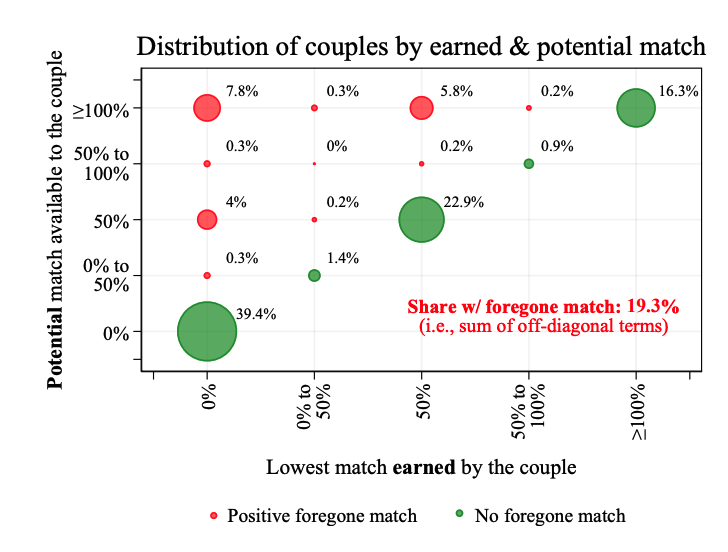
\includegraphics[width=0.9\linewidth]{inputs/figure2a.png}
\end{figure}
\end{frame}
%---------------------------------------------------------------------

%---------------------------------------------------------------------
\begin{frame}{Incidence and Magnitudes}
\small
\begin{figure}
\centering
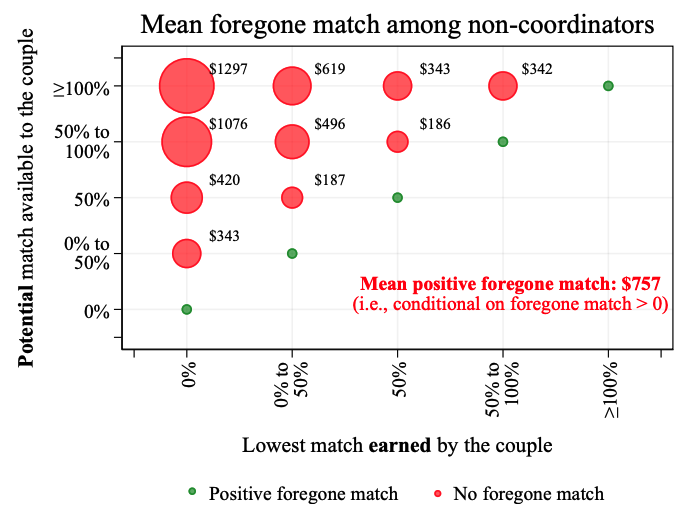
\includegraphics[width=0.9\linewidth]{inputs/figure2b.png}
\end{figure}
\end{frame}
%---------------------------------------------------------------------

%---------------------------------------------------------------------
\begin{frame}{Persistence}
\small
\begin{figure}
\centering
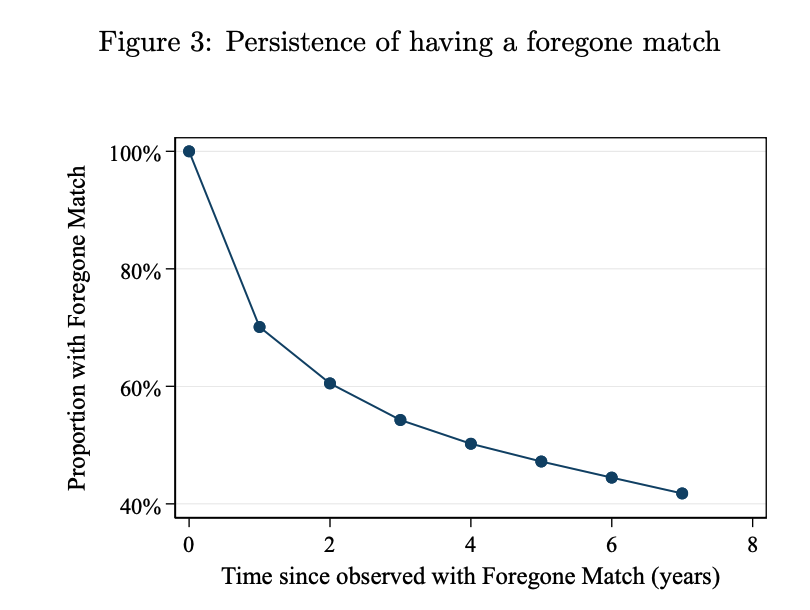
\includegraphics[width=0.7\linewidth]{inputs/fig3.png}
\end{figure}
\end{frame}
%---------------------------------------------------------------------

%---------------------------------------------------------------------
\begin{frame}{Across Demographic Groups}
\small
\begin{figure}
\centering
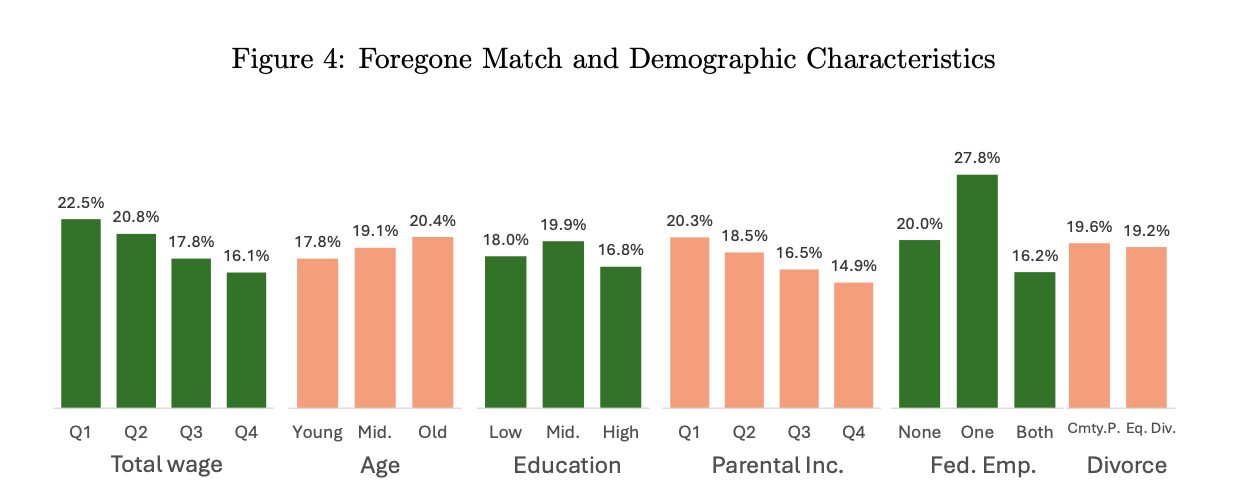
\includegraphics[width=0.9\linewidth]{inputs/fig4.png}
\end{figure}
\end{frame}
%---------------------------------------------------------------------

%---------------------------------------------------------------------
\begin{frame}{Are Couples Actively Coordinating?}
\small
\begin{itemize}
  \item Many couples with $\mathrm{FM}=0$ might simply \emph{happen} to be efficient (e.g., both fully max the match) without active coordination.
  \item Benchmark using two placebo samples with \emph{no coordination by construction}:
  \begin{itemize}
    \item \textbf{Reshuffled couples:} re-pair spouses across real couples with similar observables.
    \item \textbf{Pairs of singles:} randomly pair singles matched on observables.
  \end{itemize}
  \item In placebo samples, \textbf{33--34\%} fail the arbitrage test. Comparing to the 19.3\% in the data implies about \textbf{57--58\%} of couples are \emph{not actively coordinating}.
\end{itemize}
\end{frame}
%---------------------------------------------------------------------

%---------------------------------------------------------------------
\begin{frame}{Are Couples Actively Coordinating?}
\small
\begin{figure}
\centering
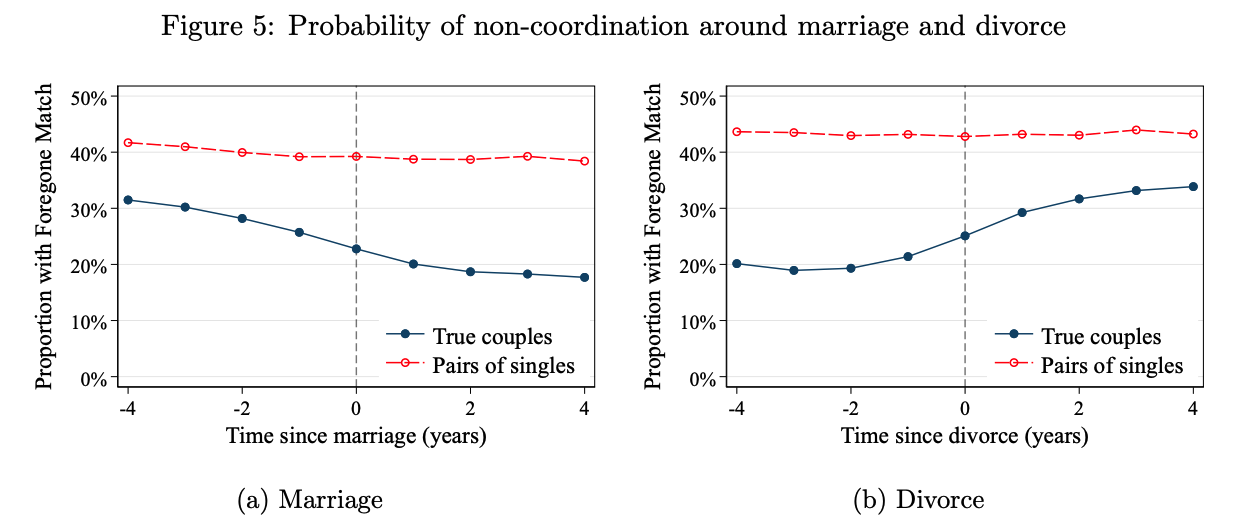
\includegraphics[width=0.9\linewidth]{inputs/fig5.png}
\end{figure}
\end{frame}
%---------------------------------------------------------------------

%---------------------------------------------------------------------
\begin{frame}{Stakes and Lifecycle Costs}
\small
\begin{itemize}
  \item \textbf{High stakes:} Non-coordination persists even when $>\$6{,}000$ (about $5\%$ of joint earnings) is at stake.
  \item \textbf{Lifecycle:} Simulation calibrated to transitions in $\mathrm{FM}>0$ and match amounts implies \textbf{$\approx\$13{,}800$--\$14{,}000} lower wealth at retirement (age 65) absent coordination.
\end{itemize}
\end{frame}
%---------------------------------------------------------------------

%---------------------------------------------------------------------
\begin{frame}{Stakes are not high enough?}
\small
\begin{figure}
\centering
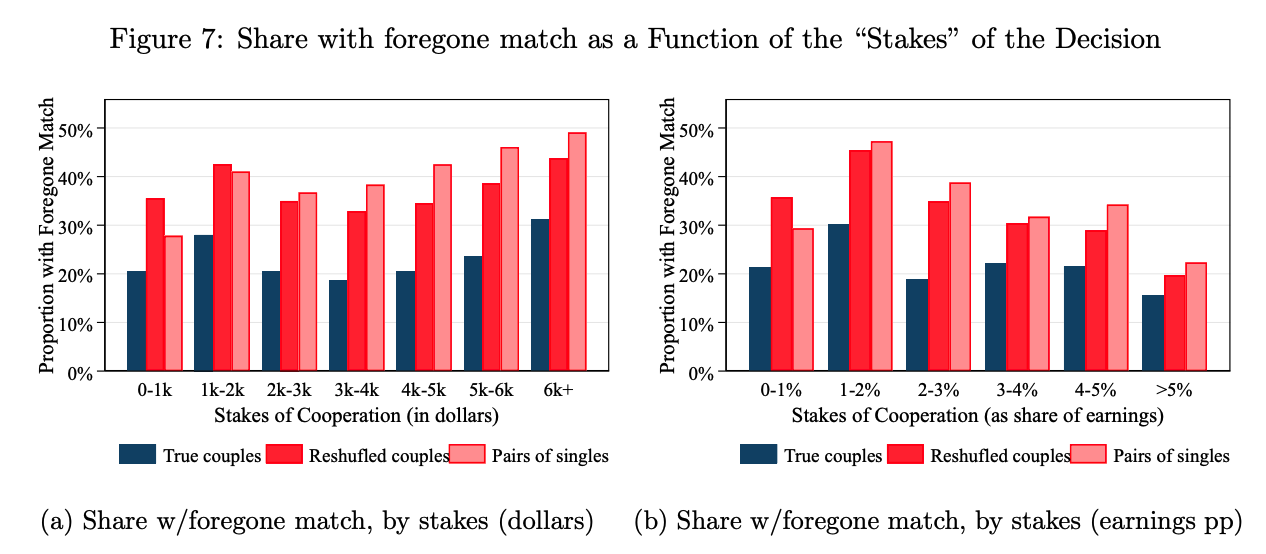
\includegraphics[width=0.9\linewidth]{inputs/fig7.png}
\end{figure}
\end{frame}
%---------------------------------------------------------------------

\subsection{Mechanisms}

%---------------------------------------------------------------------
\begin{frame}{Not (Just) Inertia or Simple Heuristics}
\small
\begin{itemize}
  \item Couples do \textbf{not} become more efficient in years when they make active saving decisions $\Rightarrow$ weak role for default inertia.
  \item A common heuristic---\textbf{equalizing contributions across spouses}---actually \emph{facilitates} efficiency rather than drives inefficiency.
  \item Non-coordination persists even with \textbf{large stakes} $\Rightarrow$ not (rational) inattention to tiny amounts.
  \item Foregone match is \textbf{less common} when both spouses work for the \textbf{same employer} (household dimension more salient).
\end{itemize}
\end{frame}
%---------------------------------------------------------------------

%---------------------------------------------------------------------
\begin{frame}{Survey Evidence: Design}
\small
\begin{itemize}
  \item Online survey of \textbf{1{,}000} working, married respondents with DC plans (Prolific).
  \item Core vignette: allocate \$3{,}000 between own vs spouse's account given two match schedules.
  \item Three randomized versions: \textit{Max via spouse}, \textit{Max via own}, \textit{Max via split}.
  \item Follow-ups elicit whether foregone match was \textbf{accidental} vs \textbf{deliberate}; measure \textbf{financial literacy} and beliefs about \textbf{asset division at divorce}.
\end{itemize}
\end{frame}
%---------------------------------------------------------------------

%---------------------------------------------------------------------
\begin{frame}{Survey Evidence: Results}
\small
\begin{itemize}
  \item \textbf{40\%} choose allocations with foregone match in the vignette.
  \item Roughly \textbf{half} of foregone match is \textbf{deliberate}, half \textbf{accidental}.
  \item Deliberate foregone match is \textbf{much higher} when maximizing requires putting \emph{all funds in the spouse's account}.
  \item \textbf{Financial literacy gradient:} foregone match falls sharply with correct answers on 5 literacy questions.
  \item \textbf{Awareness:} many couples had \emph{not considered} that coordination could increase the match.
  \item \textbf{Divorce beliefs:} over a third think they would keep their own accounts on divorce; those respondents are \textbf{more likely} to forego match.
\end{itemize}
\end{frame}
%---------------------------------------------------------------------

%---------------------------------------------------------------------
\begin{frame}{Financial literacy matters}
\small
\begin{figure}
\centering
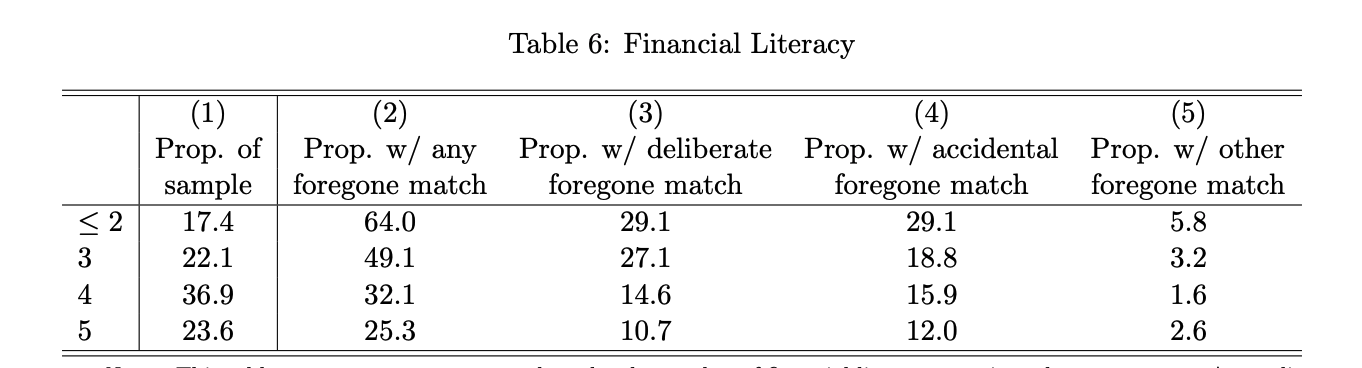
\includegraphics[width=0.9\linewidth]{inputs/table6.png}
\end{figure}
\end{frame}
%---------------------------------------------------------------------

%---------------------------------------------------------------------
\begin{frame}{Administrative Proxies for Commitment}
\small
\begin{itemize}
  \item Foregone match is \textbf{higher} among couples who later \textbf{divorce}.
  \item Foregone match is \textbf{lower} among couples who used a \textbf{joint bank account before marriage}.
  \item Other proxies: longer marriage, presence of children, and having a mortgage are associated with \textbf{more coordination}.
\end{itemize}
\end{frame}
%---------------------------------------------------------------------

%---------------------------------------------------------------------
\begin{frame}{Commitment seems to be an issue}
\small
\begin{figure}
\centering
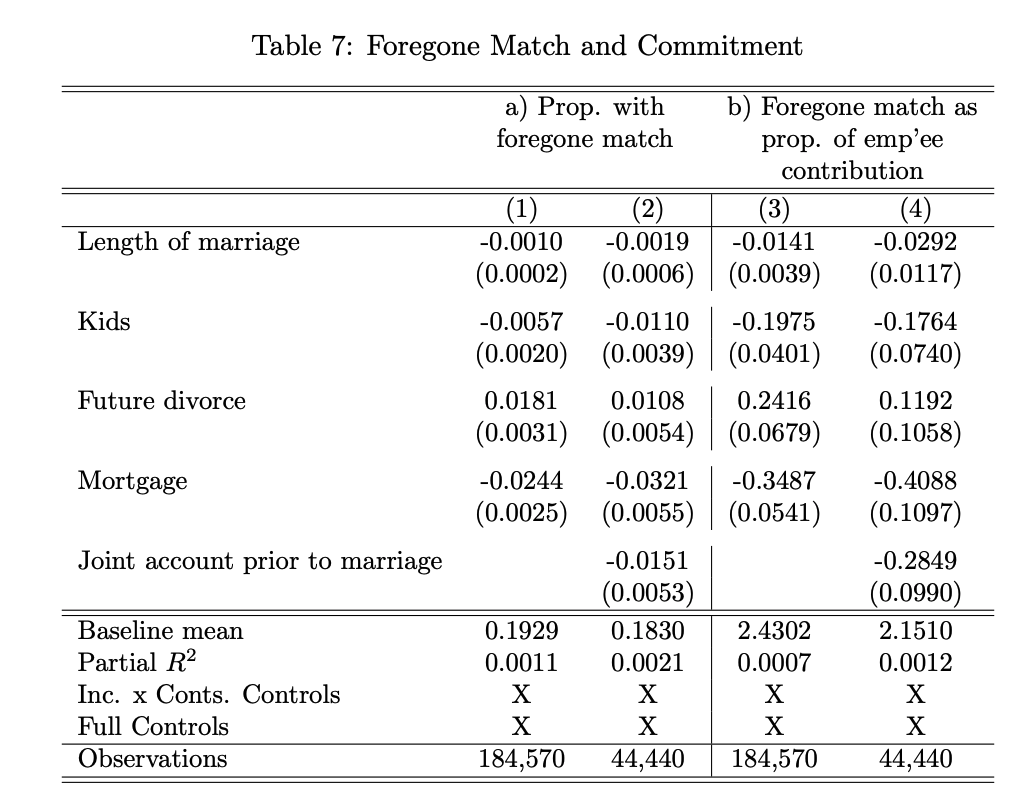
\includegraphics[width=0.9\linewidth]{inputs/table7.png}
\end{figure}
\end{frame}
%---------------------------------------------------------------------

%---------------------------------------------------------------------
\begin{frame}{As well as knowledge about divorce laws}
\small
\begin{figure}
\centering
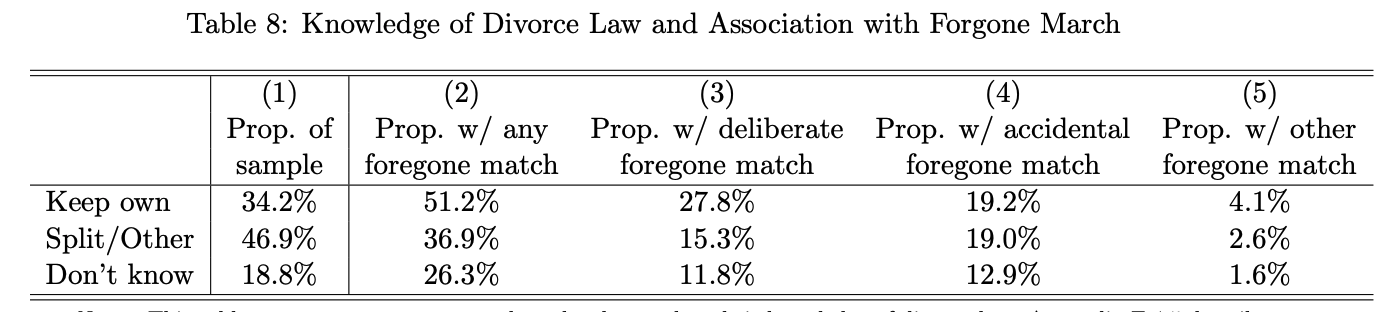
\includegraphics[width=0.9\linewidth]{inputs/table8.png}
\end{figure}
\end{frame}
%---------------------------------------------------------------------

%---------------------------------------------------------------------
\begin{frame}{Gender dynamics}
\small
\begin{figure}
\centering
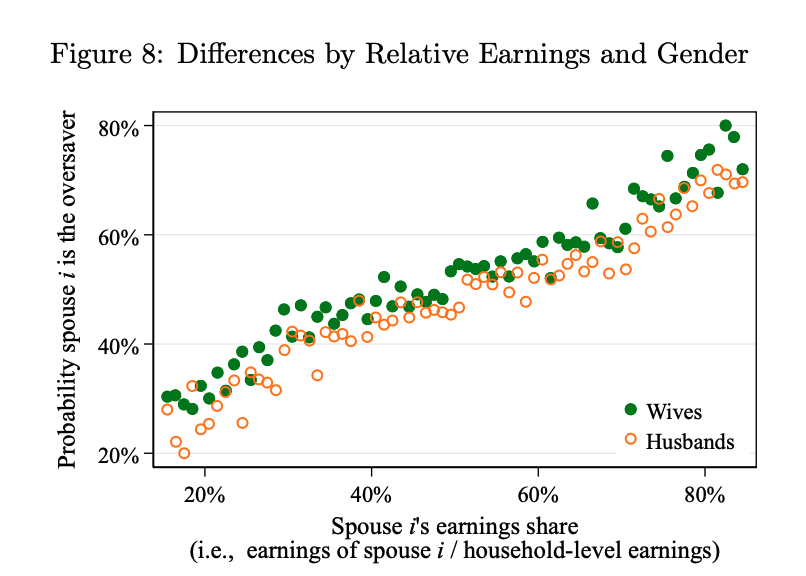
\includegraphics[width=0.7\linewidth]{inputs/fig8.png}
\end{figure}
\end{frame}
%---------------------------------------------------------------------

\subsection{Implications and Discussion}

%---------------------------------------------------------------------
\begin{frame}{Discussion}
\small
\begin{itemize}
  \item What does this evidence imply for \textbf{unitary} and \textbf{collective} models of the household? 
  \item How might \textbf{commitment frictions} or \textbf{limited attention} generate the patterns observed?
  \item Which \textbf{policy lever} would you implement, and why?
\end{itemize}
\end{frame}
%---------------------------------------------------------------------

%---------------------------------------------------------------------
\begin{frame}{Implications for Policy and Plan Design}
\small
\begin{itemize}
  \item \textbf{Default design:} auto-allocate the first dollars to the higher marginal match account (with easy opt-out).
  \item \textbf{Information:} nudge emails and on-portal alerts when one spouse is above cap while the other has match available.
  \item \textbf{Legal literacy:} improve communication about division of retirement assets upon divorce.
\end{itemize}
\end{frame}
%---------------------------------------------------------------------


% %---------------------------------------------------------------------
% \begin{frame}{Reference}
% \small
% Choukhmane, Taha; Lucas Goodman; and Cormac O'Dea (2023, rev. 2025). \emph{Efficiency in Household Decision Making: Evidence from the Retirement Savings of U.S. Couples.} NBER Working Paper No. 31195. \\
% Link: \href{https://www.nber.org/papers/w31195}{\texttt{https://www.nber.org/papers/w31195}}
% \end{frame}
% %---------------------------------------------------------------------

% =====================================================
\section{Gender Identity \& Relative Income (Bertrand--Kamenica--Pan)}

%---------------------------------------------------------------------
\begin{frame}{Today's Paper}
\textbf{Bertrand, Kamenica, \& Pan (QJE 2015; NBER WP 19023).}\\
\emph{Gender Identity and Relative Income within Households}.\\[0.5em]
\small
\begin{itemize}
  \item \textbf{Question:} Do gender norms against wives outearning husbands shape marriage, labor supply, and allocations?
  \item \textbf{Key norm:} ``A man should earn more than his wife.''
  \item \textbf{Design:} Descriptive \& quasi-experimental evidence using Census/ACS, SIPP, Canadian tax data, ATUS, NSFH.
  \item \textbf{Links:} \href{https://academic.oup.com/qje/article-abstract/130/2/571/2330321}{QJE 2015}
\end{itemize}
\end{frame}
%---------------------------------------------------------------------

%---------------------------------------------------------------------
\begin{frame}{Stylized Fact: Sharp Drop at 50\%}
Distribution of the wife's share of household labor income shows a \textbf{sharp drop just to the right of 0.5} (wife earns more than husband).\\[0.4em]
\begin{figure}
\centering
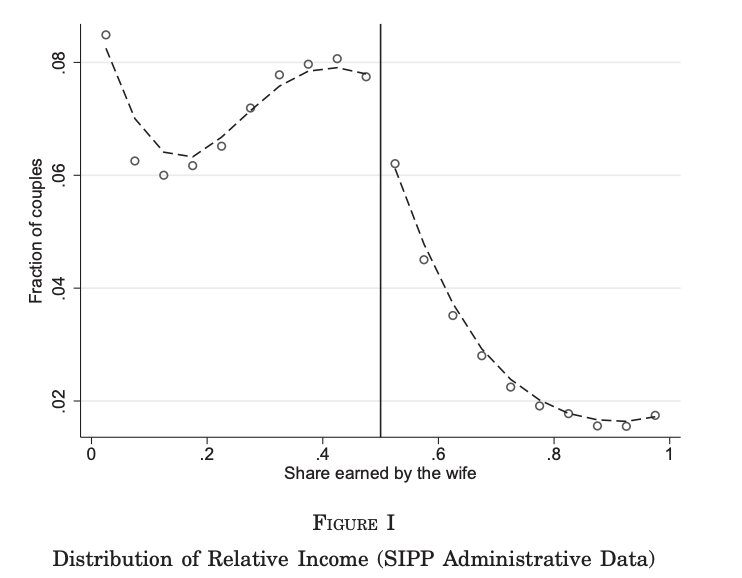
\includegraphics[width=0.5\linewidth]{inputs/paper2_fig1.png}
\end{figure}
\end{frame}
%---------------------------------------------------------------------

%---------------------------------------------------------------------
\begin{frame}{Marriage-Market Evidence}
\small
\begin{itemize}
  \item Construct \textbf{marriage markets} by age $\times$ race $\times$ education $\times$ state; compute $Pr(\text{Woman earns more than Man})$.
  \item \textbf{Result:} Marriage rates decline as this probability rises; authors attribute about \textbf{23\%} of the 1970--2010 decline in marriage to this channel.
  \item Intuition: identity-based preferences lower match surplus when wife would outearn husband.
\end{itemize}
\end{frame}
%---------------------------------------------------------------------

%---------------------------------------------------------------------
\begin{frame}{Within-Couple Labor Supply Distortions}
\small
\begin{itemize}
  \item For each married woman, estimate distribution of \textbf{potential income} from demographics; compute $Pr(\text{Wife potential} > \text{Husband actual})$.
  \item \textbf{Participation:} Higher probability $\Rightarrow$ lower labor-force participation (large negative coefficients).
  \item \textbf{Conditional earnings:} If she works, the gap between realized and potential income is larger $\Rightarrow$ \emph{under-earning}.
  \item Controls: husband income (flexibly), wife potential-income vigintiles, demographics, year \& state FE; robustness to alternative constructions.
\end{itemize}
\end{frame}
%---------------------------------------------------------------------

%---------------------------------------------------------------------
\begin{frame}{Marital Satisfaction, Divorce, and Time Use}
\small
\begin{itemize}
  \item \textbf{NSFH:} Couples with wife$>$husband income report \textbf{lower marital satisfaction} and \textbf{more marital trouble}; higher \textbf{divorce} likelihood.
  \item \textbf{ATUS:} When wife earns more, the \textbf{gender gap in home production widens}—wives do even \emph{more} housework (``compensatory'' behavior).
  \item Effects concentrate in \textbf{chores} rather than childcare.
\end{itemize}
\end{frame}
%---------------------------------------------------------------------

%---------------------------------------------------------------------
\begin{frame}{Interpretation \& Alternative Explanations}
\small
\begin{itemize}
  \item Paper’s view: \textbf{gender-identity} norm (``a man should earn more...'') fits the facts across data sources.
  \item \textbf{Misreporting?} Unlikely — administrative data (US SIPP; Canada LAD) show the same drop at 0.5.
  \item Cross-country evidence is mixed; some replications find attenuated discontinuities. 
\end{itemize}
\end{frame}
%---------------------------------------------------------------------

% =====================================================
\section{Credit, Household Bargaining, and Access (Kim, SSRN 3962414)}

%---------------------------------------------------------------------
\begin{frame}{Today's Paper}
\textbf{Kim (2021, rev. 2023).} \emph{Credit and the Family: The Economic Consequences of Closing the Credit Gap of U.S. Couples (SSRN 3962414).}\\[0.4em]
\small
\begin{itemize}
  \item \textbf{Question:} Does expanding credit access for \emph{secondary earners} shift within-household allocation and bargaining?
  \item \textbf{Policy shock:} The \textbf{2013 TILA reversal} let card issuers consider \emph{household} income (not only the applicant’s independent income) for 21+.
  \item \textbf{Design:} Treatment \(\equiv\) \emph{equitable-distribution} (ED) states; Control \(\equiv\) \emph{community-property} (CP) states that already granted access via marital property rules.
  \item \textbf{Outcomes:} Spouse-level credit limits and consumption.
\end{itemize}
\end{frame}
%---------------------------------------------------------------------

%---------------------------------------------------------------------
\begin{frame}{Institutional Background}
\small
\begin{itemize}
  \item \textbf{TILA (Reg Z) 2013 change:} removes independent ability-to-pay requirement for 21+; issuers may use income/assets the consumer can reasonably access \(\Rightarrow\) \emph{household} income counts.
  \item \textbf{Exposure:} In \textbf{ED} states, the change \emph{raised} secondary earners' borrowing capacity. In \textbf{CP} states, division-of-property rules already implied shared access \(\Rightarrow\) \emph{minimal} effect.
  \item \textbf{Intuition:} More own credit \(\Rightarrow\) better outside option and greater control over spending \(\Rightarrow\) potential shift in \emph{bargaining power}.
\end{itemize}
\end{frame}
%---------------------------------------------------------------------

%---------------------------------------------------------------------
\begin{frame}{Identification (Matched DiD)}
\small
Compare ED vs CP states around the November 2013 reform:
\[
Y_{ist} = \alpha_i + \delta_t + \beta \cdot (\text{ED}_s \times \text{Post}_t) + X_{it}'\gamma + \varepsilon_{ist},
\]
\begin{itemize}
  \item \(Y_{ist}\): spouse-level outcomes (credit limits; consumption).
  \item \(\beta\): impact on secondary earners in ED states after reform (vs CP).
  \item \textbf{Assumptions:} common trends across ED/CP (supported by event study); matched-DiD to improve balance.
  \item \textbf{Heterogeneity:} single- vs dual-income households; baseline credit access.
\end{itemize}
\end{frame}
%---------------------------------------------------------------------

%---------------------------------------------------------------------
\begin{frame}{Data and Measurement}
\small
\begin{itemize}
  \item De-identified \textbf{JPMorgan Chase} admin data: checking, debit, credit accounts for \(\sim\)\textbf{66,200} opposite-sex couples, \textbf{2012 –2015}.
  \item \textbf{Primary vs secondary earner:} by pre-reform monthly labor income; single- vs dual-income classified from payroll deposits.
  \item \textbf{Credit access:} (i) \emph{Independent} credit = sum of limits on \emph{sole} cards; (ii) \emph{Total} credit = limits on any cards each spouse can use (primary or authorized).
  \item \textbf{Consumption:} spouse-level spending from debit/credit + checking outflows; ambiguous joint transactions split equally.
\end{itemize}
\end{frame}
%---------------------------------------------------------------------

%---------------------------------------------------------------------
\begin{frame}{Pre-Reform Facts: Intra-Household Gaps}
\small
\begin{itemize}
  \item \textbf{Credit access:} before 2013, primary earners had \(\sim\) \textbf{97\%} of \emph{accessible} credit \(\Rightarrow\) large gap.
  \item \textbf{Consumption:} primary consumed \(\sim\)\textbf{59\%}, secondary \(\sim\)\textbf{41\%} of household spending \(\Rightarrow\) \textbf{18 p.p.} gap.
  \item \textbf{Interpretation:} secondary earners had limited \emph{independent} borrowing capacity and consumed less within the household.
\end{itemize}
\end{frame}
%---------------------------------------------------------------------

%---------------------------------------------------------------------
\begin{frame}{Main Effect I: Credit Access for Secondary Earners}
\small
\begin{itemize}
  \item \textbf{Credit limits} for secondary earners \(\uparrow\) by about \textbf{\$1{,}500} after the reform in ED vs CP states (\(\approx\)\textbf{60\%} of monthly pre-reform consumption).
  \item \textbf{No crowd-out:} total household credit $\uparrow$ \(\sim\)\textbf{\$1{,}532}$\Rightarrow$ secondary earners’ gains did not reduce primary earners’ limits.
\end{itemize}
\end{frame}
%---------------------------------------------------------------------

%---------------------------------------------------------------------
\begin{frame}{Main Effect I: Credit Access for Secondary Earners}
\begin{figure}
\centering
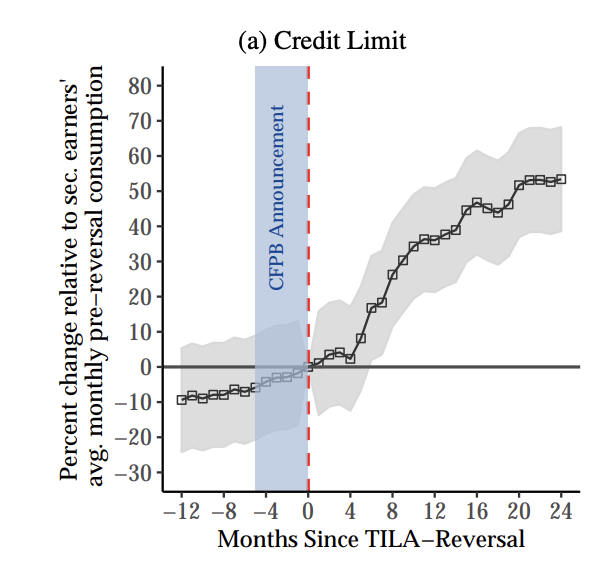
\includegraphics[width=0.5\linewidth]{inputs/paper3fig1.png}
\end{figure}
\end{frame}
%---------------------------------------------------------------------


%---------------------------------------------------------------------
\begin{frame}{Main Effect II: Consumption and Reallocation}
\small
\begin{itemize}
  \item \textbf{Consumption equalization:} spouses share consumption more equally; the pre-reform gap \textbf{closes by roughly half}.
  \item \textbf{Levels:} secondary earners’ monthly consumption \(\uparrow\) (e.g., \(\sim\)\textbf{14\%} or \(\sim\)\textbf{\$340}); household consumption \(\uparrow\) modestly (\(\sim\)\textbf{3\%} or \(\sim\)\textbf{\$170}).
  \item \textbf{Composition:} spending shifts toward goods that \emph{benefit both spouses} (shared categories).
\end{itemize}
\end{frame}
%---------------------------------------------------------------------

%---------------------------------------------------------------------
\begin{frame}{Main Effect II: Consumption}
\begin{figure}
\centering
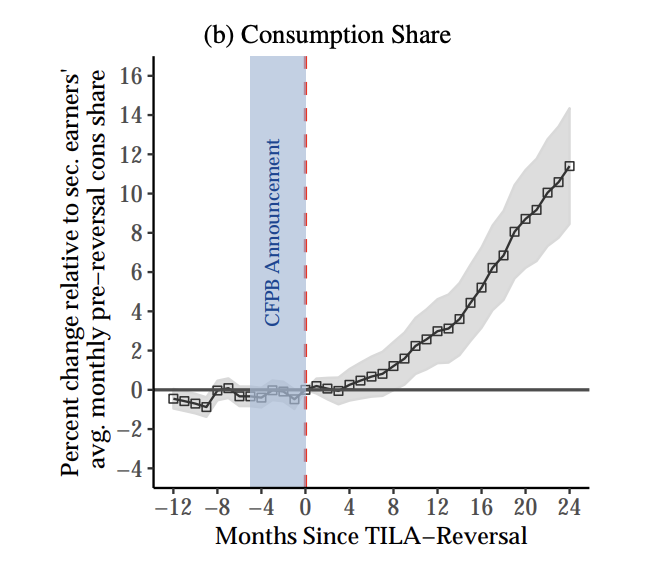
\includegraphics[width=0.5\linewidth]{inputs/paper3fig2.png}
\end{figure}
\end{frame}
%---------------------------------------------------------------------

%---------------------------------------------------------------------
\begin{frame}{Main Effect II: Reallocation}
\begin{figure}
\centering
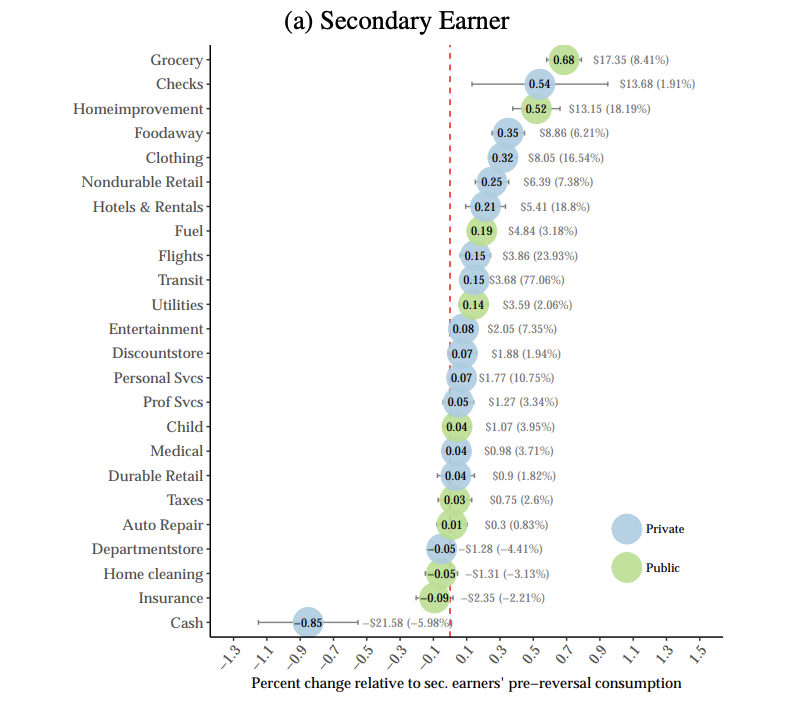
\includegraphics[width=0.5\linewidth]{inputs/paper3fig3.png}
\end{figure}
\end{frame}
%---------------------------------------------------------------------

%---------------------------------------------------------------------
\begin{frame}{Mechanisms \& Heterogeneity}
\small
\begin{itemize}
  \item \textbf{Bargaining channel:} access to one’s own credit relaxes liquidity constraints for the secondary earner \(\Rightarrow\) greater say in allocations.
  \item \textbf{Stronger effects} in \textbf{single-income} couples and for stay-at-home partners (lowest baseline independent income).
  \item \textbf{Financial health:} no measurable increase in delinquencies/overdrafts \(\Rightarrow\) improved intra-household equity without distress.
\end{itemize}
\end{frame}
%---------------------------------------------------------------------

%---------------------------------------------------------------------
\begin{frame}{Policy Implications}
\small
\begin{itemize}
  \item \textbf{Underwriting at the household margin} can reduce intra-household inequality when legal rights allow access.
  \item \textbf{Equity + prudence:} expanded access for secondary earners did \emph{not} worsen solvency—useful for regulators and issuers.
\end{itemize}
\end{frame}
%---------------------------------------------------------------------

% =====================================================
\section{Wrapping Up}

%---------------------------------------------------------------------
\begin{frame}{Conclusion: Three Views of Intra-Household (In)Efficiency}
\small
\begin{itemize}
  \item \textbf{Institutions \(\Rightarrow\) bargaining (Kim 2024):} Expanding \emph{secondary earners’} credit access shifts consumption toward equity without hurting solvency.
  \item \textbf{Norms \(\Rightarrow\) choices (BKP 2015):} Identity costs around “who earns more” shape marriage, labor supply, and time use (even with similar aggregates).
  \item \textbf{Friction \(\Rightarrow\) missed arbitrage (CGO 2023):} Many couples fail a simple \emph{static efficiency} test (employer match arbitrage), costing lifetime wealth.
  \item \textbf{Synthesis for policy:} Design \emph{for households}, not just individuals—combine \emph{rights} (credit access), \emph{information/defaults} (retirement match prompts), and \emph{norm-aware} messaging to reduce inefficiency and inequity.
\end{itemize}
\end{frame}
%---------------------------------------------------------------------

%---------------------------------------------------------------------
\begin{frame}
\begin{center}{\LARGE See you next time!}\end{center}
\end{frame}
%---------------------------------------------------------------------

% \beginbackup
% \appendix
% \input{sections/appendix.tex}
% \bibliographystyle{../bib/aeanobold}
% \nobibliography{../bib/bib.bib}
% \backupend

\end{document}
